\documentclass[tikz,border=8pt]{standalone}
% Shared look for every TikZ diagram. Load with % Shared look for every TikZ diagram. Load with % Shared look for every TikZ diagram. Load with \input{../../tools/tikz-style.tex}
\usepackage[T1]{fontenc}
\usepackage{lmodern}
\renewcommand{\sfdefault}{lmr}  % diagrams use the same serif as the text
\usetikzlibrary{arrows.meta, positioning, shapes.geometric, calc, fit, backgrounds}
\definecolor{cblue}{HTML}{4C78A8}
\definecolor{corange}{HTML}{F58518}
\definecolor{cgreen}{HTML}{54A24B}
\definecolor{cred}{HTML}{E45756}
\definecolor{cpurple}{HTML}{B279A2}
\definecolor{cgrey}{HTML}{6B6B6B}
\tikzset{
  every picture/.style={font=\sffamily, line width=1.2pt},
  box/.style={draw=#1, fill=#1!12, rounded corners=4pt, align=center, inner sep=7pt, minimum height=1.1cm},
  box/.default=cgrey,
  arrow/.style={-{Stealth[length=3mm]}, draw=cgrey, line width=1.4pt},
  title/.style={font=\sffamily\bfseries\Large},
  note/.style={font=\sffamily\small, text=cgrey, align=center},
}
\AtBeginDocument{\hyphenpenalty=10000 \exhyphenpenalty=10000}

\usepackage[T1]{fontenc}
\usepackage{lmodern}
\renewcommand{\sfdefault}{lmr}  % diagrams use the same serif as the text
\usetikzlibrary{arrows.meta, positioning, shapes.geometric, calc, fit, backgrounds}
\definecolor{cblue}{HTML}{4C78A8}
\definecolor{corange}{HTML}{F58518}
\definecolor{cgreen}{HTML}{54A24B}
\definecolor{cred}{HTML}{E45756}
\definecolor{cpurple}{HTML}{B279A2}
\definecolor{cgrey}{HTML}{6B6B6B}
\tikzset{
  every picture/.style={font=\sffamily, line width=1.2pt},
  box/.style={draw=#1, fill=#1!12, rounded corners=4pt, align=center, inner sep=7pt, minimum height=1.1cm},
  box/.default=cgrey,
  arrow/.style={-{Stealth[length=3mm]}, draw=cgrey, line width=1.4pt},
  title/.style={font=\sffamily\bfseries\Large},
  note/.style={font=\sffamily\small, text=cgrey, align=center},
}
\AtBeginDocument{\hyphenpenalty=10000 \exhyphenpenalty=10000}

\usepackage[T1]{fontenc}
\usepackage{lmodern}
\renewcommand{\sfdefault}{lmr}  % diagrams use the same serif as the text
\usetikzlibrary{arrows.meta, positioning, shapes.geometric, calc, fit, backgrounds}
\definecolor{cblue}{HTML}{4C78A8}
\definecolor{corange}{HTML}{F58518}
\definecolor{cgreen}{HTML}{54A24B}
\definecolor{cred}{HTML}{E45756}
\definecolor{cpurple}{HTML}{B279A2}
\definecolor{cgrey}{HTML}{6B6B6B}
\tikzset{
  every picture/.style={font=\sffamily, line width=1.2pt},
  box/.style={draw=#1, fill=#1!12, rounded corners=4pt, align=center, inner sep=7pt, minimum height=1.1cm},
  box/.default=cgrey,
  arrow/.style={-{Stealth[length=3mm]}, draw=cgrey, line width=1.4pt},
  title/.style={font=\sffamily\bfseries\Large},
  note/.style={font=\sffamily\small, text=cgrey, align=center},
}
\AtBeginDocument{\hyphenpenalty=10000 \exhyphenpenalty=10000}

\begin{document}
\begin{tikzpicture}[x=1.5cm, y=0.9cm]
  \node[title] at (3.6,6.6) {Variance: the average squared distance from the mean};
  \draw[cred, dashed] (3,-0.6) -- (3,5.6) node[above, font=\sffamily\small, text=cred] {mean $\bar{x} = 3$};
  \node[font=\sffamily\bfseries\small, text=cgrey] at (7.6,5.3) {distance};
  \node[font=\sffamily\bfseries\small, text=cgrey] at (8.9,5.3) {squared};
  \foreach \v/\r in {3/4, 2/3, 1/2, 5/1, 4/0} {
    \pgfmathtruncatemacro{\d}{\v-3}
    \pgfmathtruncatemacro{\s}{\d*\d}
    \draw[cgrey!50, line width=0.6pt] (0,\r) -- (6,\r);
    \ifnum\d=0 \else \draw[arrow, draw=cblue] (3,\r) -- (\v,\r); \fi
    \fill[black] (\v,\r) circle (3pt);
    \node[font=\sffamily\small, anchor=east] at (-0.1,\r) {$x = \v$};
    \node[font=\sffamily] at (7.6,\r) {$\d$};
    \node[font=\sffamily] at (8.9,\r) {$\s$};
  }
  \foreach \t in {0,...,6} \node[font=\sffamily\small, text=cgrey] at (\t,-0.9) {\t};
  \draw[cgrey] (7.1,-0.5) -- (9.4,-0.5);
  \node[font=\sffamily] at (7.6,-0.95) {sum $0$};
  \node[font=\sffamily] at (8.9,-0.95) {$10$};
  \node[font=\sffamily] at (3.6,-2.6) {$\sigma^2 = \dfrac{0 + 1 + 4 + 4 + 1}{5} = \dfrac{10}{5} = 2$};
\end{tikzpicture}
\end{document}
